%!TEX root = main.tex


\section{Basics of Finite Volume Method}

\begin{frame}{Principles of Finite Volume Method}
Firstly, here is a concise introduction to the finite volume method. 
% If you think that is too simple and all audience can understand, just tell me and I would skip.

For the typical equation in the fluid dynamics,
\begin{equation}
\frac{\partial u}{\partial t}+\nabla \cdot \Gamma=F \text { in } \Omega
\end{equation}

Except for the finite difference method which is not compatible with the unstructured mesh, finite volume and finite element are introduced here. These two methods play the role of transforming operators (differentiate, divergence) into discretized parts of an equation. 



\end{frame}

\begin{frame}{Principles of Finite Volume Method}
On the base of the typical equation, a test funciton is multiplied on both sides and the equation is integrated on a specific region, hence,
\begin{equation}
\int_{\Omega} \frac{\partial u}{\partial t} \varphi d V+\int_{\Omega}(\nabla \cdot \Gamma) \varphi d V=\int_{\Omega} F \varphi d V
\end{equation}

By Gauss theorem and integrating by parts, 
\begin{equation}
\int_{\Omega} \frac{\partial u}{\partial t} \varphi d V-\int_{\Omega} \Gamma \cdot \nabla \varphi d V+\int_{\partial \Omega} \Gamma \cdot \mathbf{n} \varphi d S=\int_{\Omega} F \varphi d V
\end{equation}
How to pick the test function and choose the integration region decides whether it is finite volume or finite element method.


\end{frame}

\begin{frame}{Principles of Finite Volume Method}
\begin{equation*}
\int_{\Omega} \frac{\partial u}{\partial t} \varphi d V-\int_{\Omega} \Gamma \cdot \nabla \varphi d V+\int_{\partial \Omega} \Gamma \cdot \mathbf{n} \varphi d S=\int_{\Omega} F \varphi d V
\end{equation*}
In the \alert{finite volume method}, one uses a constant function $1$ directly and integrate the equation on each cell. For each cell, one conservative variable corresponds to an equation. The second term of the function is omitted. The total equation number is nearly $Cell\ Number * Variable\ Number$, the same as FEM.  

While in the \alert{finite element method}, state variables are stored in the nodes of the grid. The integration region is defined as the neighboring region around the node. The test function is chosen to be zero on the boundary of the region so that the third term of the equation is omitted in internel cells.
\end{frame}
\begin{frame}{Principles of Finite Volume Method}
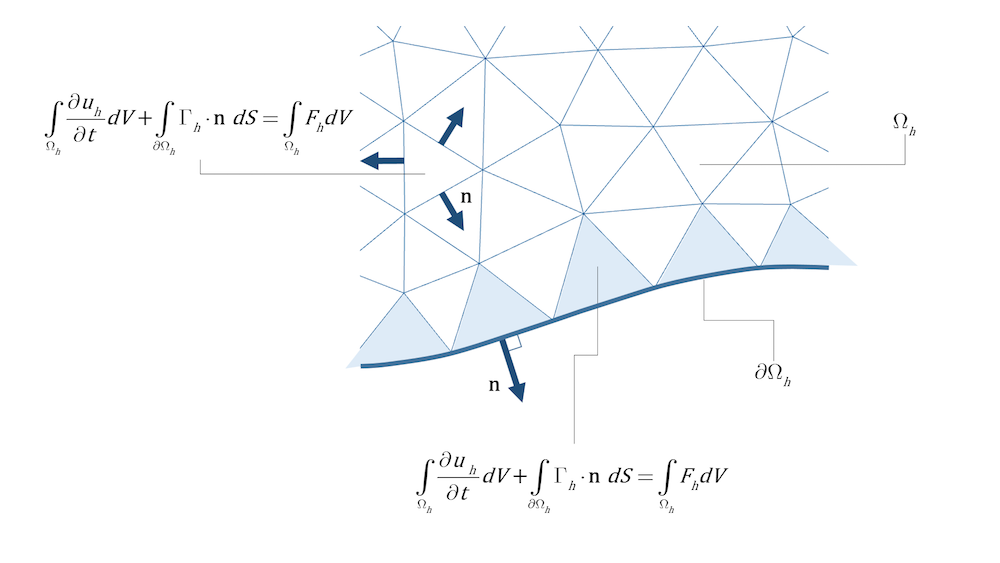
\includegraphics[width=\linewidth]{figures/integrated-flux-internal-cells.png}\\
Finite Volume Method Integration Region Diagram
\end{frame}

\begin{frame}{Principles of Finite Volume Method}
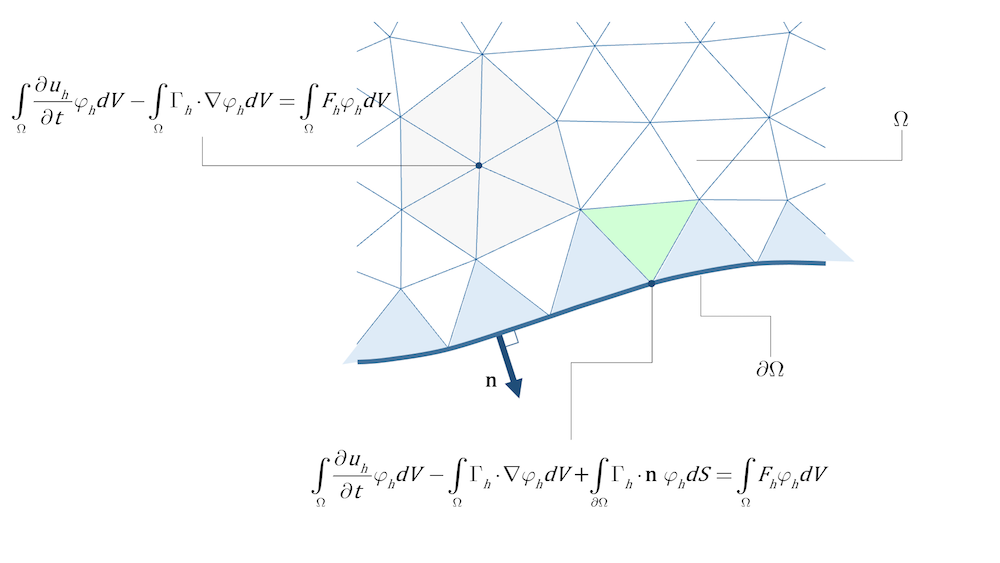
\includegraphics[width=\linewidth]{figures/domain-contribution-internal-elements.png}\\
Finite Element Method Integration Region Diagram
\end{frame}


\begin{frame}[allowframebreaks]
\frametitle{Comparison among CFD and MHD Code}
\footnotesize{\tiny}

\begin{center}
\begin{tabular}{l >{\ttfamily}c >{\ttfamily}c >{\ttfamily}c >{\ttfamily}c}
\toprule
Code & Frame & Institute & Field & Model for MHD \\
\midrule
SU2\footnote{SU2, Stanford University Unstructured \parencite{SU2EconomonIntro}} & FVM/FEM & Stanford U.(open) & CFD &-\\
JOREK & FEM & EUROfusion &   Fusion & 2-fluid \\
M3D-C1\footnote{\textcite{M3DC1:Web}} & FEM & PPPL & Fusion& 2-fluid \\
FLASH &  &  \\
PLUTO & FVM/FDTD & Torino U.(open) & Aero & 1-fluid (RMHD)\\
\bottomrule
\end{tabular}
\end{center}

\begin{center}
\begin{tabular}{l >{\ttfamily}c >{\ttfamily}c >{\ttfamily}c >{\ttfamily}c}
\toprule
Code & Grid & Adaptive Grid & $\cdots$ & $\cdots$ \\
\midrule
SU2 & Unstructured & Support \\
JOREK & Flux-aligned & - & \\
M3D-C1 & Unstructured &\\
FLASH &  &  \\
PLUTO & Structured & Support &\\
\bottomrule
\end{tabular}
\end{center}
\end{frame}

\begin{frame}{Comparison among CFD and MHD Code}
\footnotesize

The most two popular codes in CFD are (1) openFOAM and (2) SU2, in which openFOAM is too large and old for an application in the future. Considering the following points, \alert{SU2} is adopted as the final choice of my research.  

There are some requirements for the research,
\begin{description}
    \item[Modularized]The equations can be coupled flexibly. Especially for multiphysics application, e.g. the plasma-wall interaction is sometimes needed while sometimes omitted for saving time.
    \item[Modern]It would save a lot of time if no fortran embedded.
    \item[Unstructured]Due to the geometry of torus, the grid arrangement is essential for the computation accuracy. Even the flux-aligned 2D Bezier finite element in JOREK may be not precise enough to capture instabilities during the double nut merging due to the flux-aligned grid only has one center. 
    \item[Adaptive Mesh]An adaptive mesh will not only make the result more accurate, but also save tremendous computation resources from those grids which change not so quickly.
\end{description}


\end{frame}


\begin{frame}{JOREK and M3D-C1 Mesh}
\begin{figure}
\begin{minipage}[t]{0.5\linewidth}
\centering
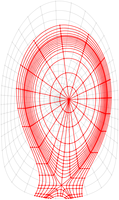
\includegraphics[width=1.2in]{figures/grid_xpoint_medium.png}
\caption{JOREK Mesh}
% \label{fig:side:a}
\end{minipage}%
\begin{minipage}[t]{0.5\linewidth}
\centering
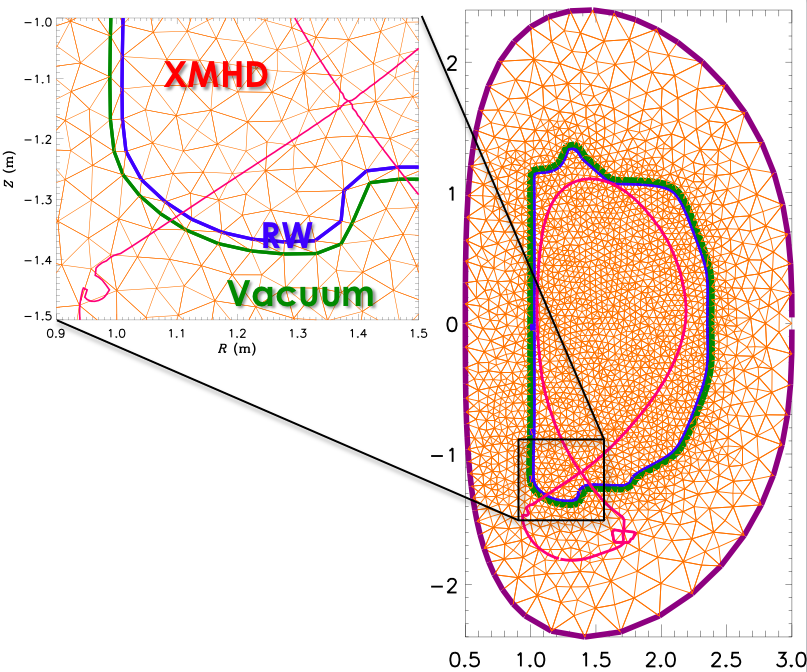
\includegraphics[width=1.8in]{figures/M3D_C1_resistive_wall.png}
\caption{M3D-C1 Mesh}
% \label{fig:side:b}
\end{minipage}
\end{figure}
    
\end{frame}

\begin{frame}{Adaptive Mesh in SU2}
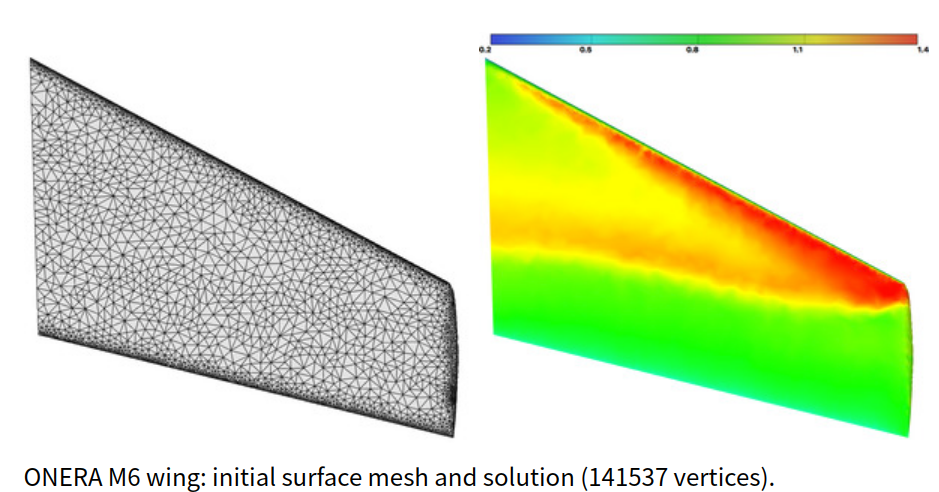
\includegraphics[width=\linewidth]{figures/ONERA_Wing_Initial_Mesh.png}
\end{frame}

\begin{frame}{Adaptive Mesh in SU2}
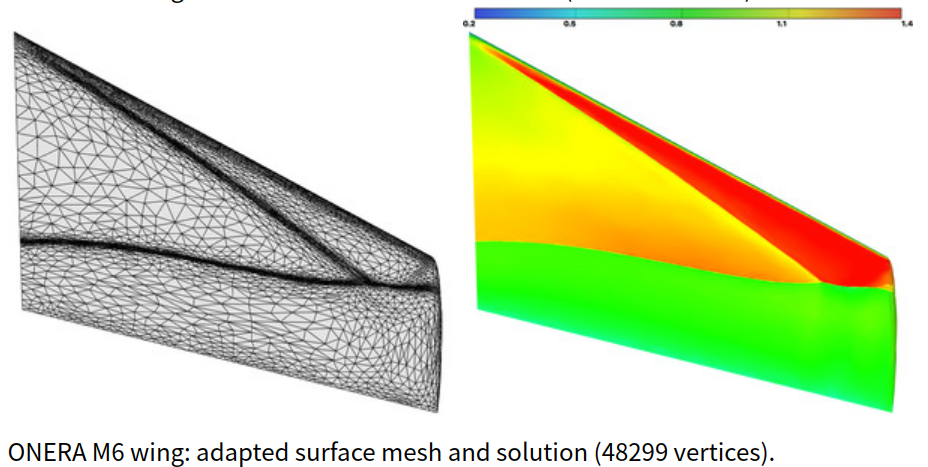
\includegraphics[width=\linewidth]{figures/ONERA_Wing_Adapted_Mesh.png}
\end{frame}

\subsection{Physics of Codes}

\begin{frame}{Physics of Codes, M3D-C1}
Firstly, a set of fluid equations,
\begin{equation}
\begin{aligned} \frac{\partial n}{\partial t}+\nabla \cdot(n \vec{u})=& 0 \\ n m_{i}\left(\frac{\partial \vec{u}}{\partial t}+\vec{u} \cdot \nabla \vec{u}\right)=& \vec{J} \times \vec{B}-\nabla p-\nabla \cdot \Pi+\vec{F} \\ \frac{\partial p}{\partial t}+\vec{u} \cdot \nabla p+\Gamma p \nabla \cdot \vec{u}=&(\Gamma-1)\left[Q-\nabla \cdot \vec{q}+\eta J^{2}-\vec{u} \cdot \vec{F}-\Pi : \nabla u\right] \\ &+\frac{1}{n e} \vec{J} \cdot\left(\frac{\nabla n}{n} p_{e}-\nabla p_{e}\right)+(\Gamma-1) \Pi_{e} : \nabla\left(\frac{1}{n e} \vec{J}\right) \\ \frac{\partial p_{e}}{\partial t}+\vec{u} \cdot \nabla p_{e}+\Gamma p_{e} \nabla \cdot \vec{u}=&(\Gamma-1)\left[Q_{e}-\vec{q}_{e}+\eta J^{2}-\vec{u} \cdot \vec{F}_{e}-\Pi_{e} : \nabla u\right] \\ &+\frac{1}{n e} \vec{J} \cdot\left(\frac{\nabla n}{n} p_{e}-\nabla p_{e}\right)+(\Gamma-1)\left[\Pi_{e} : \nabla\left(\frac{1}{n e} \vec{J}\right)+\frac{1}{n e} \vec{J} \cdot \vec{F}_{e}\right] \end{aligned}
\end{equation}

Generalized Ohm's law,
\begin{equation}
\vec{E}=-\vec{u} \times \vec{B}+\eta \vec{J}+\frac{1}{n e}\left(\vec{J} \times \vec{B}-\nabla p_{e}-\nabla \cdot \Pi_{e}+\vec{F}_{e}\right)
\end{equation}

A reduced set of Maxwell's equations,
\begin{equation}
\begin{aligned} \vec{J} &=\frac{1}{\mu_{0}} \nabla \times \vec{B} \\ \frac{\partial \vec{B}}{\partial t} &=-\nabla \times \vec{E} \end{aligned}
\end{equation}
\end{frame}

\begin{frame}{Physics of Codes, JOREK}

2-fluid MHD model is probably a too large topic to talk about in this presentation, because it is not the focus of the presentation.

Here we have the resitivity MHD model in JOREK as an example.

\alert{Resitivity MHD model},
\begin{equation}
\left\{
\begin{array}{l}
{\partial_{t} \rho+\nabla \cdot(\rho \boldsymbol{v})=0} \\ 
{\rho \partial_{t} \boldsymbol{v}+\rho \boldsymbol{v} \cdot \nabla \boldsymbol{v}+\nabla(p)=\boldsymbol{J} \times \boldsymbol{B}+\nabla \cdot(\nu \nabla \boldsymbol{v})} \\ 
{\partial_{t} p+\boldsymbol{v} \cdot \nabla p+\gamma p \nabla \cdot \boldsymbol{v}=0} \\ {\partial_{t} \boldsymbol{B}=-\nabla \times \boldsymbol{E}=\nabla \times(\boldsymbol{v} \times \boldsymbol{B}-\eta \boldsymbol{J})} \\ {\nabla \times \boldsymbol{B}=\boldsymbol{J}} \\ {\nabla \cdot \boldsymbol{B}=0}\end{array}\right.
\end{equation}

Be careful of the degenerative Maxwell:
\begin{itemize}
    \item $\boldsymbol{J}$ is decided by the curl of magnetic field here, which means $\boldsymbol{E}$ is much more stable than $\boldsymbol{B}$.
    \item Time derivative of $p$ is replaced by the energy derivative in fluid dynamics SU2. 
\end{itemize}


\end{frame}


\begin{frame}{Physics of Codes, SU2}


\begin{equation*}
\frac{\partial U}{\partial t}+\nabla \cdot \vec{F}^{c}-\nabla \cdot\left(\mu^{v k} \vec{F}^{v k}\right)=Q \quad \text { in } \Omega, t>0
\end{equation*}


\begin{equation*}
U=\left\{\begin{array}{c}{\rho } \\ {\rho \vec{v} } \\ {\rho E}\end{array}\right\},\quad
\vec{F}^{c}=\left\{\begin{array}{c}{\rho \vec{v}} \\ {\rho \vec{v} \otimes \vec{v}+\overline{\overline{I}} p} \\ {\rho E \vec{v}+p \vec{v}}\end{array}\right\}
\end{equation*}

\begin{equation*}
\vec{F}^{v1}=\left\{\begin{array}{c}{\cdot} \\ {\overline{\overline{\tau}}} \\ {\overline{\overline{\tau}}\cdot \vec{v}}\end{array}\right\},\quad
\vec{F}^{v2}=\left\{\begin{array}{c}{\cdot} \\ {\cdot} \\ {c_p \nabla T}\end{array}\right\},\quad
Q=\left\{\begin{array}{c}{q_\rho} \\ {\vec{q}_{\rho\vec{v}}} \\ {q_{\rho E}}\end{array}\right\}
\end{equation*}

\end{frame}

\begin{frame}{Conservative Equations}
\begin{equation}
\frac{\partial \boldsymbol{U}}{\partial t}+\underbrace{\nabla \cdot \boldsymbol{F}^{c}}_{\text CONV\ TERM}-\overbrace{\nabla \cdot\left(\mu^{v k} \boldsymbol{F}^{v k}\right)}^{\text VISC\ TERM}=\boldsymbol{Q} \quad \text { in }\Omega,  \quad t>0
\end{equation}

Most SU2 scripts are located in the \textit{SU2\_CFD} and \textit{Common} folder, other folders contain very limited amount of codes concerning adaptive mesh, dual grid and \textit{e.t.c.} 

\begin{itemize}
    \item OS: Cross-platform
    \item Lang: C++, Python
    \item Mainly vertex-based dual mesh FVM, also supports FEM and primal grid
\end{itemize}
\end{frame}

\begin{frame}{SU2 Framework}
\uncover<+->{\begin{equation*}
\frac{\partial U}{\partial t}+\nabla \cdot \vec{F}^{c}-\nabla \cdot\left(\mu^{v k} \vec{F}^{v k}\right)=Q \quad \text { in } \Omega, t>0
\end{equation*}
}
\uncover<+->{\[ \Downarrow \]
\begin{align*}
    \int_{\Omega_{i}} \frac{\partial U}{\partial t} d \Omega & + \sum_{j \in \mathcal{N}(i)}\left(\tilde{F}_{i j}^{c}+\tilde{F}_{i j}^{v k}\right) \Delta S_{i j}-Q\left|\Omega_{i}\right| \\ 
=\int_{\Omega_{i}} \frac{\partial U}{\partial t} d \Omega & +  R_{i}(U)=0
\end{align*}
}

For each variable in each cell, there is a residual.
\end{frame}



% \subsection{Temporal Discretization}
\begin{frame}{Temporal Discretization}
The requirement of temporal discretization in Maxwell equations is no different from others.

Explicit RK,
\begin{equation}
\left\{\begin{array}{l}{u^{(1)}=u^{n}} \\ {u^{(2)}=u^{n}+\alpha_{2} d t F\left(u^{(1)}\right)} \\ {u^{(3)}=u^{n}+\alpha_{3} d t F\left(u^{(2)}\right)} \\ {\cdots} \\ {u^{(k)}=u^{n}+\alpha_{k} d t F\left(u^{(k-1)}\right)} \\ {u^{n+1}=u^{n}+d t \sum_{j=1}^{q} \beta_{j} F\left(u^{(j)}\right)}\end{array}\right.
\end{equation}

Implicit RK and dual time stepping \parencite{SU2LiDualTime} are also available in SU2, and compatible with the Maxwell equations.
\end{frame}





% \begin{frame}[fragile,allowframebreaks]
% \frametitle{Java Code Sample}
    
% \begin{lstlisting}[language=Java,basicstyle=\ttfamily\footnotesize,gobble=8,
%     emph={parse,lp,typedDependenciesCCprocessed,lemmaStatic,dep,gov,reln,index,tag,value},
%     morekeywords={TreebankLanguagePack,GrammaticalStructureFactory,GrammaticalStructure,
%         List,TypedDependency,IndexedWord,String,Morphology},
%         escapechar=|]
%         // Continue from earlier Java code 
%         // Use the parsed tree to get the typed dependencies
%         TreebankLanguagePack tlp = lp.treebankLanguagePack();
%         GrammaticalStructureFactory gsf = tlp.grammaticalStructureFactory();
%         GrammaticalStructure gs = gsf.newGrammaticalStructure(parse);
%         List<TypedDependency> tdl = gs.typedDependenciesCCprocessed();

%         // Let's just print out each of the parent-child relationship first
%         for (TypedDependency td : tdl) {
%             // parent = "governer"
%             IndexedWord parent = td.gov();
%             String parentWord = parent.value();
%             String parentPOS = parent.tag();
%             String parentLemma = Morphology.lemmaStatic(
%                 parentWord, parentPOS, true);
            
%             |\framebreak|
%             // child = "dependent"
%             IndexedWord child = td.dep();
%             String childWord = child.value();
%             String childPOS = child.tag();
%             String childLemma = Morphology.lemmaStatic(
%                 childWord, childPOS, true);
            
            
%             System.out.println(
%                 "[" + parent.index() + "]" + parentLemma + "/" + parentPOS 
%                 + " <--" + td.reln().getShortName() + "-- "
%                 + "[" + child.index() + "]" + childLemma + "/" + childPOS);
%         }
%         System.out.println();
% \end{lstlisting}

% \end{frame}




